\chapter{绪\hspace{6pt}论}

\section{课题研究背景及意义}
合成孔径雷达(Synthetic Aperture Radar, SAR)作为一种对地成像雷达,通过搭载在飞机或卫星上实现对地物目标测量。与传统的光学传感器件相比,SAR探测成像不受时间、气候等因素的影响,具有全天时、全天候的成像特点,可以实现持续对地物目标的探测\citing{皮亦鸣2007合成孔径雷达成像原理}。全极化SAR作为SAR系统的子类,通过发射接收不同极化方式的电磁波信号,实现对地物目标散射信息的探测。相比于传统的SAR系统,极化SAR数据具有更丰富的散射特征,蕴含更多的目标信息。目前,由于极化SAR的多极化特性,极化SAR技术已经成为合成孔径雷达技术中不可或缺的分支。在极化SAR的众多应用中,极化SAR图像解译工作已经成为其中最重要的研究方向之一,目的是快速、准确地获取极化SAR图像中的地物目标信息,在军事目标探测、城市规划、灾害估计等多个军事民事领域已经得到了广泛应用\citing{甘甜2015面向对象的高分辨率遥感影像建筑物震害信息提取}。

极化SAR图像分类技术在解读极化SAR数据方面扮演着重要的角色。其核心在于特征提取和目标分类方法等技术的实施。可靠的地物目标分类结果依赖于合理且有效的特征提取工程和目标分类方法,才能充分体现出极化SAR复杂探测数据的重要价值。由于极化SAR的多极化成像特性,极化SAR图像中具备了丰富的极化信息,而这些信息的发现与利用需要借助有效的极化特征表示方法。特征表示是极化SAR图像解译中最基本、最关键的步骤,对最终的分类结果具有重要的影响。利用合理的特征表示,能够使分类模型更加快速、准确的迭代到最优参数,取得优秀的分类结果;反之,不合理的特征表示即便是使用更加复杂的分类器模型,也很难达到出色的分类结果。极化SAR图像的目标分类算法也属于解译的关键步骤,其本质是为极化SAR图像中的每一个像素赋予合理的类别。目标分类算法旨在确定一个非线性的分类规则,将所有具有相似特征的样本划分为同一类别,而将不相似特征的样本归为不相同的类别。有效分类同类和异类地物目标是分类器设计的关键所在。

近年来,相比于极化SAR成像能力方面的持续进步和显著发展,极化SAR图像解译技术的提升较为缓慢,这也导致了极化SAR在实际工程中应用的限制。首先,由于成像系统分辨率的提升,虽然为地物目标带来更加丰富的细节信息,,但同时也为极化SAR图像解译工作带来了新的阻碍。其次,随着对极化SAR图像特征表征技术的研究发展,涌现了越来越多的极化特征,这些特征从多个不同的角度对地物目标进行描述,如何合理且全面地利用这些极化特征也称为极化SAR图像解译的难题。最后,随着极化SAR技术的不断发展,获取到的极化SAR数据集呈现爆炸性增长趋势,但是标记这些数据集依赖专业知识,需要较大的人工成本和精确的标注技术,由于人工标记错误、自动标记技术精度不足等因素导致的错误标记样本问题给极化SAR图像解译带来巨大的困难\citing{tu2020robust,uhlmann2013integrating,liu2016large}。因此如何利用混杂有噪声标签的有限标记的数据集也成为极化SAR图像解译中的新挑战。具体而言,体现在:

(1)极化SAR图像表现出高分辨率趋势,其中具有更加丰富的地物散射信息。目前,极化SAR特征提取技术发展迅猛,极化特征提取方法日渐增多,这些方法从不同的角度对地物目标的散射特性进行描述。然而,当前大多数的极化SAR图像分类算法仅仅采用了单一类型的极化特征。然而,对于空间环境复杂的场景,具有更复杂的集合结构。单一类型的极化特征无法全面地描述目标的细节信息,无法对目标信息进行全面概括。同时,固定的极化特征表示方式无法在所有类型的地物目标和图像中取得满意的结果。

(2)极化SAR技术不断发展,极化SAR数据集数量呈现爆发式增长。对极化SAR数据集的标注工作依赖专业知识或自动标注技术,由于极化SAR的复杂成像特性,标注工作中不可避免地由于人工错误标记、自动标注技术精度不足等问题出现错误标记的样本。如何高效的利用混杂有噪声样本的数据集是当前极化SAR图像分类研究的难点。

本文旨在利用深度学习技术优势,基于地物目标的散射特性差异,探索极化SAR图像的极化特征最优表征方式。同时利用深度学习技术优势,实现在混杂有噪声样本的有限数据集中的可靠分类,提高极化SAR图像的分类准确率,进而提升极化SAR系统的实际可用性。

\section{国内外相关研究现状}
极化SAR图像分类技术中包含两个关键步骤,即极化特征表示和分类器的设计。本文的研究内容致力于极化特征的表示方法和分类器设计方法。因此,将从极化特征表示和目标分类方法这两个方面来进行现状分析。

\subsection{极化特征表示方法}
极化SAR图像中蕴含了丰富的极化信息,而这些信息的发现和应用都依赖于有效的极化特征表示方法。极化特征表示在极化SAR图像解译任务中扮演着至关重要的基础角色。

像素作为极化SAR图像的基本组成单元,现有的大多数极化SAR图像特征表示和分类方法都是以像素为最小单元进行处理,也就是利用每个像素点本身的特征来完成特征表示和分类。一般而言,常见的极化特征表示方法有对观测数据进行简算数运算构造的特征、基于极化目标分解理论的目标分解特征、图像空间纹理特征等。

(1)对观测数据进行算数运算构造的特征

极化SAR图像的观测数据是指以极化散射矩阵、经过多视处理的相干矩阵和协方差矩阵为代表的相关数据。通过对这些观测数据进行简单的代数运算可以得到用于表征地物部分散射特性的简单特征,主要包括观测数据的相位、幅度以及对应的四则运算等。Rignot等人\citing{rignot1992unsupervised}提出了使用极化协方差矩阵中的各个元素的对数来实现极化SAR图像的分割;Pierce等人\citing{pierce1994knowledge}结合极化散射矩阵和专家系统展开了对极化SAR图像的分类研究;Kong等人\citing{1988Identification}提出了利用极化散射矩阵每个通道的强度之比来进行极化SAR图像分类研究工作;Lee等人\citing{2001Quantitative}使用散射矩阵计算出相位差,结合最大似然分类器进行分类;Ding等人\citing{1017062722.nh}从散射矩阵和相干矩阵中的各个元素组成特征向量,用于分类研究。基于观测数据简单代数运算的特征简单易得,属于最基本的极化特征,但是缺少了对地物目标的具体物理散射机制的深层解释。

(2)基于极化目标分解理论的目标分解特征

极化目标分解理论通过从物理意义层面对极化SAR数据进行约束,来反映地物目标确切物理意义的散射特性,是极化SAR数据利用中最为经典且至关重要的理论之一。Huynen在1970年首次提出了目标分解理论\citing{huynen1970phenomenological,huynen1990stokes},为后续研究工作奠定了理论基础。极化目标分解按照处理的数据不同,可以分为极化相干分解和极化非相干分解两种方式。极化相干分解的处理对象是散射矩阵,利用不同的基将散射矩阵分解为多个具有不同物理意义的矩阵分量的加权和的形式。极化非相干分解的处理对象是相干矩阵或协方差矩阵,也是将其分解为多个具有不同物理意义的分量的加权和的形式。

极化相干分解针对散射矩阵数据,从物理层面进行约束,利用不同的基向量将散射矩阵分解为不同物理意义的矩阵分量加权和。经典的极化相干分解方法包括Pauli分解\citing{cloude1996review}、Krogager分解\citing{krogager1990new}、Cameron分解\citing{cameron1990feature}等。Puali分解方法是将散射矩阵分解为单次散射、方向角为0°和45°的二次散射的组合;Krogager分解则是将散射矩阵分解为球散射、二面角散射和螺旋体散射的组合形式;Cameron分解基于Pauli分解方法,提出了对定向角旋转之后的最大散射成分作为分解特征的方法。相干分解要求目标具有稳定的散射性质和相干的散射波,适用于没有噪声的环境,对于存在一个主要目标的场景效果优越,能够准确地表达地物目标的物理散射特性。

极化非相干分解方法针对多视矩阵的数据处理,将其分解为多个反映确切物理意义的参数加权和的形式。经典的非相干分解方法包括Cloude分解\citing{cloude1997entropy}、Freeman分解\citing{freeman1998three}、Holm分解\citing{holm1988radar}等。Cloude分解方法利用矩阵的特征值理论,基于矩阵的最大特征值来推断目标的散射类型,还提出了一系列的散射特征,包括散射熵、各项异度性和平均散射角等极化特征;Freeman分解属于基于模型的分解方法,按照地物目标的散射差异,分为平面散射、二次散射和体散射三种类型,其中平面散射主要出现在表面光滑的地物区域,二次散射主要出现在城市区域,尤其是密集建筑物群的地域,体散射主要发生在森林、灌木从等植被茂密区域。

目标分解理论为极化SAR数据处理提供了一系列具有特定物理含义的极化特征,从不同的角度反映的地物目标的物理散射特性,是当前极化SAR特征提取领域最为重视、应用最为广泛的方法。一般而言,通过一种目标分解方法,可以得到1至4个对应的特征参数,而不同的目标分解方法能从不同的角度反映地物的散射机制和地物类型。在某些复杂的地形场景中,不同的目标可能会产生不同的散射回波,相同类型地物目标也有可能产生不同的回波\citing{tu2011laplacian}。因此,采用单一的极化特征描述方法往往无法获得理想的结果。

(3)图像空间纹理特征

在极化SAR图像分类领域,空间纹理特征作为极化特征的补充表示,是对地物目标空间细节特性描述的重要特性之一。直方图统计、Gabor滤波、小波变换等空间纹理特征提取方法在图像解译领域发挥了重要作用。Haralick等人\citing{haralick1973textural}基于灰度共生概率的纹理特征来对SAR图像分类,并通过实验证实了方案可行性;Fauvel等人\citing{fauvel2008spectral}通过基于形态学的高光谱高分辨城市图像分类方法与支持向量机(Support Vector Machine,SVM)相结合的形式,通过以上形态学方法,有效的提升了分类准确率;He等人\citing{he2013texture}结合小波信息与稀疏编码进行特征提取,以SVM作为分类器完成极化SAR图像分类;Ji等人\citing{ji2015segmentation}则结合局部二值模式和HSV空间的颜色特征完成极化SAR图像分类任务。尽管空间纹理特征作为一种易于实现的补充特征在极化SAR图像特征提取领域取得了良好的表现,但是提取范围通常收到尺度限制,无法自适应的对尺度进行缩放而导致分类精度受到限制。


\subsection{极化SAR目标分类方法}
极化SAR图像分类方法作为极化SAR图像解译的关键步骤之一\citing{},受到了国内外诸多研究学者的关注和重视。极化SAR图像分类任务本质是将图像中的每一个像素规矩分类规则赋予一个类别标签,确定所属的地物类别。图\ref{fig:极化SAR分类流程}展示了极化SAR图像数据处理以及目标分类方法的基本流程,整个流程包括极化SAR数据处理、极化特征表示、样本预处理、分类方法四个步骤。其中,目标分类方法是通过对输入极化SAR数据样本的学习,形成按照样本特征进行分类的规则,根据分类规则对剩下的测试样本完成目标分类的流程。当前的极化SAR图像分类算法根据训练过程中使用人工标记样本的数量情况可以分为无监督分类、有监督分类和半监督分类三种类型。

\begin{figure}[h]
    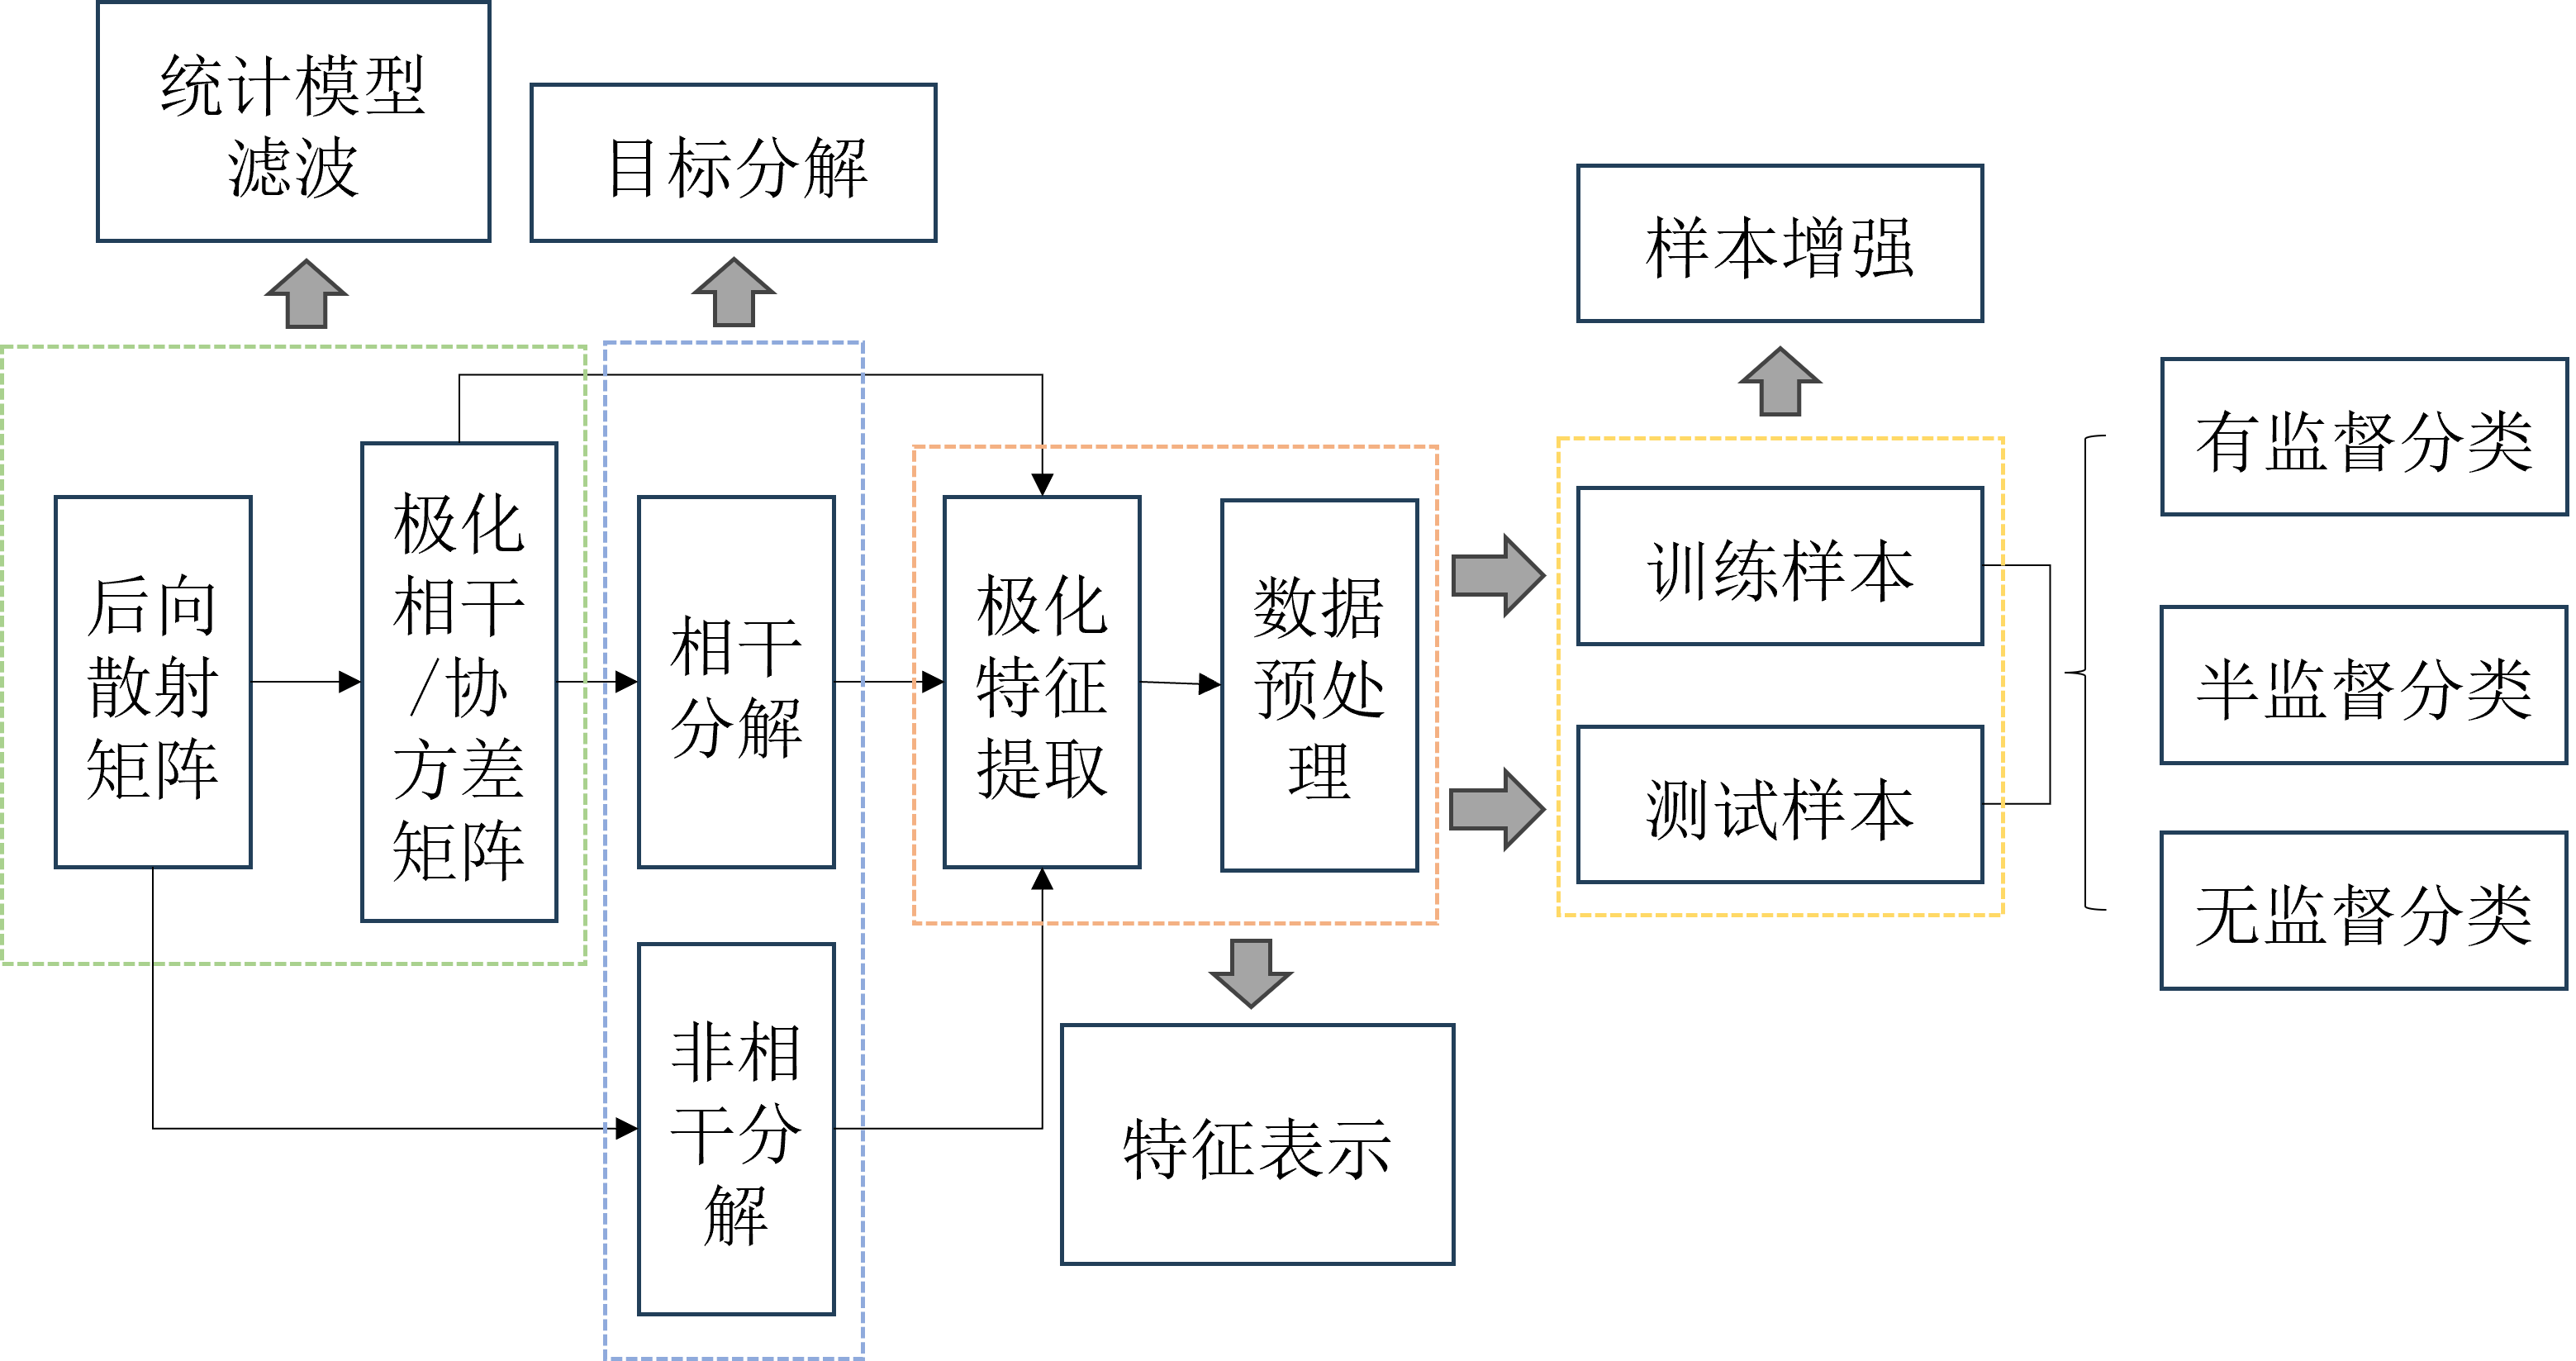
\includegraphics[width=12.3cm]{pic/chapter1/极化SAR分类流程.png}
    \caption{极化SAR分类流程}
    \label{fig:极化SAR分类流程}
\end{figure}


\subsubsection{无监督分类方法}
无监督学习分类方法是指在缺失地物标签信息的情况下完成对目标的分类任务。极化SAR无监督分类任务中,主要是依据极化SAR数据的内在不同特征分布情况,来区分不同类型的地物目标,并且最终每个类别的标签需要人工进行标注。Van Zyl等人提出了基于入射、反射波之间关系的分类准则,并且首次将极化SAR的目标散射特性运用到目标分类方法中\citing{};Cloude等人创新性地提出了极化熵$\mathrm{H}$以及平均散射角$\bar{\alpha}$的极化特征描述概念,并在$\mathrm{H}-\bar{\alpha}$平面中划分了8个代表不同散射机理的区域,来表示不同的地物类型\citing{};Lee等人在Cloude的研究基础上进一步提出了利用复Wishart分布的无监督学习方法,开创新地将地物目标物理散射特性和统计特征相结合,为后续的无监督研究工作提供了启发性的思路\citing{}。Ferro-Famil等人引入了在Cloude的研究基础上引入了各项异度性$\mathrm{A}$,并且进一步地将$\mathrm{H}-\bar{\alpha}$的8区域扩展为16个区域,使分类结果更加准确,包含更多的细节\citing{};Yamaguchi等人将散射总功率SPAN与分类方法相结合,获得更好收敛性的无监督分类方法\citing{};Lee等人在Freeman分解的基础上,将基于复Wishart分类方法与Freeman分解相结合,通过先进行模糊分类,然后进行精细分类的方式,最后利用Wishart进行迭代分类得到最终的分类结果\citing{};Bi等人提出了一种基于目标分解理论和K-Wishart似然分类方法相结合的无监督分类方法,基于Pottier和Lee\citing{}的方法先产生粗分类结果,然后利用多个不同的极化特征和K-Wishart分类方法的最大似然算法实现精确分类\citing{}。尽管无监督分类方法充分利用了极化SAR数据的目标散射特性和统计分布特性,但是由于标记样本的缺失,同物异谱和异物同谱的情况下往往分类效果较差。

\subsubsection{有监督分类方法}
相比于无监督分类方法,有监督分类方法在确定分类规则时能够使用有标签的数据来进行匹配训练,通常表现出更加优越的分类性能。基于统计理论的分类方法是极化SAR图像分类领域应用最为广泛的方法,也被成为基于贝叶斯理论的分类方法。Kong等人从极化矢量服从高斯分布这一特性出发,构建了基于复高斯分布的最大似然分类器\citing{};Lee等人利用傅相干矩阵服从Wishart分布理论基础,提出了Wishart分类器\citing{}。

除了以上提及的基于极化SAR数据分布特性的有监督分类方法,近年来,由于深度学习的自动挖掘数据鉴别特征和优越的分类性能,广泛的应用于自然语言处理、智能驾驶、信息检索等领域。由于其优越的性质,越来越多的研究将深度学习方法应用到遥感图像解译领域中,也获得了巨大的成果。Lv等人将深度信念网络(Deep Belief Network, DBN)应用到极化SAR图像分类中,并取得了优异的分类效果\citing{};Xie等人利用堆叠式自编码器(Stacked Sparse Autoencoder, SSAE)来获取可鉴别特征,随后基于标签微调,实现了分类性能和区域分类视觉效果上的巨大提升\citing{}。Zhou等人使用一维向量来表征极化SAR数据的相干矩阵,并将其作为CNN的输入作为分类,开创性地将卷积网络分类方法引入到极化SAR图像分类中\citing{}。Zhang等人在Zhou的研究基础上提出了基于复数的卷积网络结构(Complex-valued CNN, CV-CNN),通过将卷积网络中的基本模块,包括卷积层、池化层、激活函数、全连接层等均扩展至复数的形式,并且提出了适用于复数域的反向传播优化算法,进一步提升了CNN在极化SAR图像分类任务中的分类准确率\citing{},并且为后续的一系列复数域分类算法奠定了基础\citing{}。现有的基于深度学习的极化SAR图像分类算法中,大多数是将极化SAR观测数据的散射矩阵或相干矩阵直接作为网络的输入,而没有充分利用现有的多种类型的极化特征,并且提取的特征缺乏物理意义。因此,如何利用深度网络来有效探索极化SAR的可鉴别特征仍然需要进一步的研究。

\subsubsection{半监督分类方法}
半监督的分类学习方法是同时利用有标签样本数据和无标签样本数据对分类模型进行训练的方法,属于有监督学习方法和无监督学习方法的有效融合。实际上,在遥感数据中,尤其是SAR数据,要获得大量的标记样本往往是非常困难的,有标记样本数量有限,而无标记的样本大量存在,并且包含了极化SAR数据分布的特征。因此,如何利用大量的无标签数据和少量的标记样本来辅助网络学习到更加准确的分类规则,已经成为一个研究重点。Liu等人\citing{}通过建图的方法,利用选定的锚点来构建邻接矩阵,实现从有标签样本到无标签样本的标签传播;Hou等人\citing{}基于字典学习和区域一致特性,学习到稀疏的高级特征之后结合无标签样本实现分类器的训练;Jie等人\citing{}基于超像素方法来应对极化SAR中存在的相干斑噪声的问题;Liu等人\citing{}和Liu等人\citing{}利用无标签样本数据,通过生成对抗网络学习到数据的分布特性,实现生成样本扩充训练集数量。

\section{论文主要内容及章节安排}
针对极化SAR分辨率提升、噪声标签必然存在的情况下的极化SAR图像分类性能提升问题,本文开展了基于极化SAR图像特征表示和目标分类的相关研究,重点研究关于极化特征融合。本文共分为五个章节,各章节结构安排为:

第一章:绪论。阐述本文工作的研究背景与意义,并且对其中的极化特征提取、极化SAR目标分类方法进行国内外研究现状进行概括分析,最后给出全文的结构安排。

第二章:极化SAR领域理论基础。首先介绍了电磁波与极化的描述方法,随后对极化SAR的数据表征方式进行了详细介绍,包括散射数据表征方式和几种经典的目标分解理论。

第三章:基于双通道注意力的极化信息提取方法。

第四章:

第五章:对本文研究工作进行总结,并展望未来工作。